\documentclass{article}
\usepackage[utf8]{inputenc}
\usepackage[spanish]{babel}
\usepackage{graphicx}
\usepackage{geometry}
\usepackage{enumerate}
\usepackage{titlesec}
\usepackage{float}
\usepackage{listings}
\usepackage{xcolor}
\usepackage{amsmath}
\usepackage{matlab-prettifier}
\usepackage{tabularx}

\geometry{letterpaper, margin = 1.5cm}

\newcommand{\codefontsize}{\fontsize{10}{11}}
\lstset{
	style = Matlab-editor,
	basicstyle = \codefontsize\ttfamily,
	mlshowsectionrules = true,
	upquote = true,
	tabsize = 4,
	captionpos = b,
	breaklines = true,
	breakatwhitespace = true,
	frame = single,
}

%Datos de la Portada
\title{Introducción a la Programación \ Practica 3}
\author{Medina Martinez Jonathan Jason \ 2023640061}
\date{25 de marzo del 2023}

\begin{document} %Inicio del Documento
	
	\fontsize{12}{16}\selectfont
	
	\begin{figure}[t] %Logos Portada
		
		
\includegraphics[width=2.5 cm]{Logo1.jpeg}
		\hfill
		
\includegraphics[width=3 cm]{Logo2.png}
		
	\end{figure}
	
	\maketitle %Titulo Portada
	\newpage
	
	\tableofcontents %Indice
	\newpage
	
	\section{Objetivo}
	
	El objetivo de esta práctica es desarrollar funciones que puedan ser llamadas desde la ventana de comandos para convertir unidades de medida.
	
	\section{Introducción}
	
	En la práctica 4 de Herramientas Computacionales, se busca desarrollar habilidades para implementar funciones en MATLAB que puedan ser llamadas desde la ventana de comandos. Las funciones a implementar tienen distintas aplicaciones como el cálculo de la altura y masa de una persona, cálculo de la resistencia equivalente de varias resistencias en paralelo y la distancia entre un punto y una recta en el plano. Además, se deben programar distintos ejercicios en los que se aplican estas funciones y se solicita al usuario interactuar con ellas.
	
	\newpage
	\section{Desarrollo}
	
	\subsection{calc\_altura\_peso(altura\_cm, peso\_kg)}
	
	Escriba una función en MATLAB con dos argumentos de entrada y dos de salida. La función debe calcular la altura en pulgadas y la masa en libras de una persona a partir de su altura en centímetros y de su peso en kilogramos. Los argumentos de entrada de la función serán la altura en centímetros y el peso en kilogramos, y los argumentos de salida deben ser la altura en pulgadas y la masa en libras. Pruebe su función en la ventana de comandos utilizando su altura y su peso. Posteriormente, cree un programa que solicite al usuario su altura en centímetros y su peso en kilogramos y le informe al usuario la respectiva conversión.
	
	\subsubsection{Función}
	
	\begin{lstlisting}
		
		function [altura_pulgadas, peso_libras] = calc_altura_peso(altura_cm, peso_kg)
		
		% CALC_ALTURA_PESO Convierte la altura de cm a pulgadas y el peso de
		% kilogramos a libras.
		%
		% Sintaxis:
		%   [altura_pulgadas, peso_libras] = calc_altura_peso(altura_cm, peso_kg)
		%
		% Entradas:
		%   altura_cm - Altura en centimetros
		%   peso_kg - Peso en kilogramos
		%
		% Salidas:
		%   altura_pulgadas - Altura en pulgadas
		%   peso_libras - Peso en libras
		
		altura_pulgadas = altura_cm / 2.54;
		
		peso_libras = peso_kg / 2.205;
		
		end
		
	\end{lstlisting}
	
	\subsubsection{Script}
	
	\begin{lstlisting}
		
		% Este programa solicita al usuario su altura en centimetros y su peso en
		% kilogramos, y utiliza la funcion "convertir_altura_peso" para calcular su
		% altura en pulgadas y su masa en libras e imprime el resultado en la
		% pantalla.
		
		cm = input('Por favor ingrese su altura en centimetros: ');
		kg = input('Por favor ingrese su peso en kilogramos: ');
		
		[in, lb] = calc_altura_peso(cm, kg);
		
		fprintf('Su altura en pulgadas es %.2f y su masa en libras es %.2f.\n', in, lb);
	\end{lstlisting}
	\newpage
	\subsubsection{Ejecución}
	
	\begin{lstlisting}
		
	>> convertir
	Por favor ingrese su altura en centimetros: 174
	Por favor ingrese su peso en kilogramos: 80
	Su altura en pulgadas es 68.50 y su masa en libras es 36.28.
		
	\end{lstlisting}

	\subsection{fdex(x)}
	
	Escriba una función MATLAB para la siguiente función matemática:
	
	\begin{equation*}
		f(x) = 2.9x^4 + 12.5x^2 - 6*x
	\end{equation*}
	\newline
	Escriba la función de forma que $x$ pueda ser un vector. Pruebe su función en la ventana de comandos con $f(-6)$ y $f(15)$. Posteriormente, cree un programa que solicite al usuario un límite inferior $a$ y un límite superior $b$ y grafique la función $f(x)$ en el rango $a \leq x \leq b$.
	
	\subsubsection{Función}
	
	\begin{lstlisting}
		
		function y = fdex(x)
		
		% FDEX Calcula la siguiente funcion matematica:
		% fdex(x) = ((2.9*x)^4) + ((12.5*x)^2) - (6*x)
		%
		% Sintaxis:
		% y = fdex(x)
		%
		% Entrada:
		% x - El valor de la variable
		%
		% Salida:
		% y - El resultado de la funcion
		
		y = ((2.9*x).^4) + ((12.5*x).^2) - (6*x);
		
		end
		
	\end{lstlisting}
	
	\subsubsection{Script}
	
	\begin{lstlisting}
		
		% Este programa permite graficar la funcion f(x) en un rango especificado 
		% por el usuario.
		
		a = input('Ingrese el limite inferior a: ');
		
		b = input('Ingrese el limite superior b: ');
		
		x = linspace(a, b, 1000);
		
		y = fdex(x);
		
		plot(x, y, 'blue', 'LineWidth', 1.5);
		
		xlabel('x');
		
		ylabel('f(x)');
		
		title('Grafica de la funcion f(x)');
		
	\end{lstlisting}
	
	\subsubsection{Ejecución}
	
	\begin{lstlisting}
	>> programa2
	Ingrese el limite inferior a: -50
	Ingrese el limite superior b: 50
		
	\end{lstlisting}
	
	\subsubsection{Grafica}
	
	\begin{figure}[H]
		\centering
		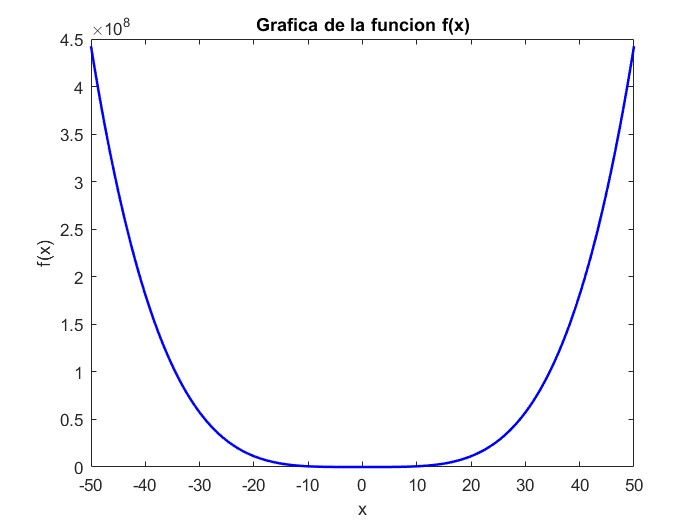
\includegraphics[width=\textwidth]{img1.jpg}
	\end{figure}
	
	\newpage
	\subsection{r(ang)}
	
	Escriba una función MATLAB para la siguiente función matemática:
	
	\begin{equation*}
		r(\theta) = 2(1.2 - \sin^2(\theta))
	\end{equation*}
	
	Escriba la función de forma que $\theta$ pueda ser un vector. Pruebe su función en la ventana de comandos con $r(\frac{\pi}{4})$ y $r(\frac{3\pi}{4})$.
	
	\subsubsection{Función}
	
	\begin{lstlisting}
		
		function y = r(ang)
		
		% Calcula la funcion r(ang) = 2(1.2 - sin^2(ang)) para un vector de
		% valores de ang
		
		y = 2*(1.2 - sin(ang).^2);
		
		end
		
	\end{lstlisting}
	
	\subsubsection{Ejecución}
	
	\begin{lstlisting}
	>> r(pi/4)
	
	ans =
	
	1.4000
	
	>> r(3*pi/4)
	
	ans =
	
	1.4000
	\end{lstlisting}
	
	Posteriormente, cree un programa que grafique la función $r(\theta)$ en el rango $0 \leq \theta \leq 2\pi$.
	
	\subsubsection{Script}
	
	\begin{lstlisting}
		
		% Este programa permite graficar la funcion r(ang) en un rango de 0 a 2pi.
		
		ang = linspace(0, 2*pi, 1000);
		
		A = r(ang);
		
		plot(ang, A, 'red', 'LineWidth', 1.5);
		
		xlabel('ang');
		
		ylabel('r(ang)');
		
		title('Grafica de r(ang)');
		
	\end{lstlisting}
	
	\subsubsection{Ejecución}
	
	\begin{lstlisting}
	>> programa3
	\end{lstlisting}
	
	\subsubsection{Grafica}
	
	\begin{figure}[H]
		\centering
		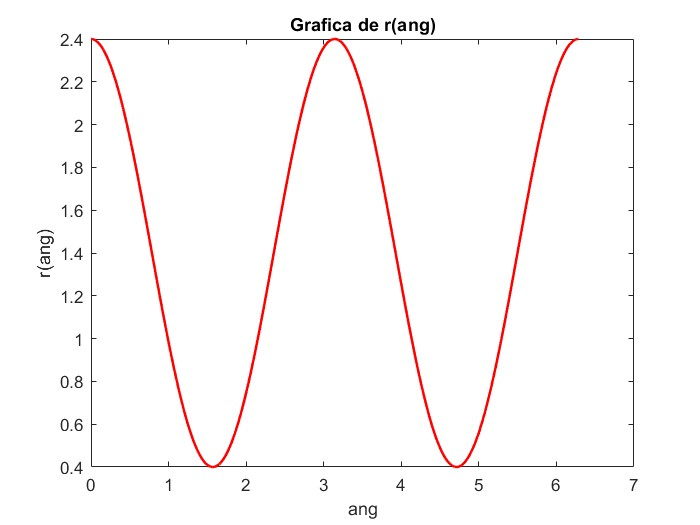
\includegraphics[width=\textwidth]{img2.jpg}
	\end{figure}
	
	\newpage
	\subsection{angulostriangulo(a, b, c)}
	
	Escriba una función que calcule los ángulos de un triángulo a partir de las longitudes de sus lados. La función deberá solicitar los tres lados $(a, b, c)$ y devolver los tres ángulos $(\alpha, \beta, \gamma)$.
	
	\subsubsection{Función}
	
	\begin{lstlisting}
		
		function [alpha, beta, gamma] = angulos_triangulo(a, b, c)
		
		% ANGULOSTRIANGULO Funcion que calcula los angulos de un 
		% triangulo a partir de las longitudes de sus lados.
		%
		% Sintaxis:
		% angulosTriangulo(a, b, c)
		%
		% Entradas:
		% a - longitud del lado a del triangulo
		% b - longitud del lado b del triangulo
		% c - longitud del lado c del triangulo
		%
		% Salida:
		% alpha - angulo opuesto al lado a en grados
		% beta - angulo opuesto al lado b en grados
		% gamma - angulo opuesto al lado c en grados
		
		alpha = acosd((b^2 + c^2 - a^2) / (2 * b * c));
		
		beta = acosd((a^2 + c^2 - b^2) / (2 * a * c));
		
		gamma = acosd((a^2 + b^2 - c^2) / (2 * a * b));
		
		end
		
	\end{lstlisting}
	
	\subsubsection{Ejecución}
	
	Pruebe su función con los siguientes datos:
		$$a = 10, b = 15, c = 7$$
	\begin{lstlisting}
	>> [a, b, c] = angulosTriangulo(10, 15, 7)
	
	a =
	
	34.0477
	
	
	b =
	
	122.8783
	
	
	c =
	
	23.0739
		
	\end{lstlisting}
	\newpage
	$$a = 6, b = 8, c = 10$$
	\begin{lstlisting}
	>> [a, b, c] = angulosTriangulo(6, 8, 10)
	
	a =
	
	36.8699
	
	
	b =
	
	53.1301
	
	
	c =
	
	90
		
	\end{lstlisting}
	$$a = 200, b = 75, c = 250$$
	\begin{lstlisting}
	>> [a, b, c] = angulosTriangulo(200, 75, 250)
	
	a =
	
	41.4096
	
	
	b =
	
	14.3615
	
	
	c =
	
	124.2289
		
	\end{lstlisting}
	
	\subsubsection{Script}
	
	Posteriormente, escriba un programa que solicite al usuario los tres lados de un triangulo y le muestra los tres angulos.
	
	\begin{lstlisting}
		% Programa para solicitar los tres lados del triangulo al usuario
		
		a = input("Ingrese el lado a: ");
		
		b = input("Ingrese el lado b: ");
		
		c = input("Ingrese el lado c: ");
		
		[alpha, beta, gamma] = angulostriangulo(a, b, c);
		
		fprintf("Los angulos del triangulo son:\n");
		
		fprintf("alpha = %.2f grados\n", alpha);
		fprintf("beta = %.2f grados\n", beta);
		fprintf("gamma = %.2f grados\n", gamma);
		
	\end{lstlisting}
	
	\subsubsection{Ejecución}
	
	\begin{lstlisting}
	>> programa4
	Ingrese el lado a: 15
	Ingrese el lado b: 20
	Ingrese el lado c: 10
	Los angulos del triangulo son:
	alpha = 46.57 grados
	beta = 104.48 grados
	gamma = 28.96 grados
	\end{lstlisting}

	\begin{lstlisting}
		>> programa4
		Ingrese el lado a: 64
		Ingrese el lado b: 78
		Ingrese el lado c: 100
		Los angulos del triangulo son:
		alpha = 39.78 grados
		beta = 51.25 grados
		gamma = 88.97 grados
	\end{lstlisting}
	
	\newpage
	
	\subsection{distancia(x0, y0, A, B, C)} 
	Escriba una función MATLAB que calcule la distancia entre un punto $(x_0, y_0)$ y una recta $$Ax + By + C = 0$$ en el plano. La función debería recibir como parámetros $x_0$, $y_0$, $A$, $B$ y $C$ y devolver la distancia $d$.
	
	\subsubsection{Función}
	
	\begin{lstlisting}
		
		function d = distancia(x0, y0, A, B, C)
		% DISTANCIA Calcula la distancia entre un punto (x0, y0) 
		% y una recta Ax + By + C = 0
		%
		% Entradas:
		% x0 - El valor de x0
		% y0 - El valor de y0
		% A - El valor de A
		% B - El valor de B
		% C - El valor de C
		%
		% Salida:
		% d - La distancia
		
		res = abs(A*x0 + B*y0 + C) / sqrt(A^2 + B^2);
		
		d = res;
		end
		
	\end{lstlisting}
	
	Pruebe su función con lo siguiente:
	
	\begin{enumerate}[]
		\item 	Punto: $(2, 4)$, recta: 
				\begin{equation*}
					y = (2x + 6)/3.5
				\end{equation*}
				\begin{lstlisting}
					>> x0 = 2;
					y0 = 4;
					A = -2/3.5;
					B = 1;
					C = 6/3.5;
					>> distancia(x0, y0, A, B, C)
					
					ans =
					
					3.9691
				\end{lstlisting}
		\item	Punto: $(11, 2)$: recta:
				\begin{equation*}
					y = - 5x + 2
				\end{equation*}
				\begin{lstlisting}
					>> x0 = 11;
					y0 = 2;
					A = -5;
					B = -1;
					C = 2;
					distancia(x0, y0, A, B, C)
					
					ans =
					
					10.7864
				\end{lstlisting}
	\end{enumerate}
	
	Posteriormente, cree un programa que solicite al usuario un punto y las constantes de la ecuación de la recta, y que le muestre en pantalla la distancia.
	
	\subsubsection{Script}
	
	\begin{lstlisting}
		%Programa que solicita los valores de x0, y0, A, B, C para calcular la 
		% distancia de unpunto a una recta de la forma Ax + By + C = 0
		
		x0 = input('Ingrese la coordenada x del punto: ');
		y0 = input('Ingrese la coordenada y del punto: ');
		
		A = input('Ingrese la constante A de la ecuacion de la recta: ');
		B = input('Ingrese la constante B de la ecuacion de la recta: ');
		C = input('Ingrese la constante C de la ecuacion de la recta: ');
		
		d = distancia(x0, y0, A, B, C);
		
		fprintf(['La distancia entre el punto (%g, %g) y la recta %gx + %gy + ' ...
		'%g = 0 es: %g\n'], x0, y0, A, B, C, d);
	\end{lstlisting}
	
	\subsubsection{Ejecución}
	
	\begin{lstlisting}
	>> programa5
	Ingrese la coordenada x del punto: 15
	Ingrese la coordenada y del punto: 10
	Ingrese la constante A de la ecuacion de la recta: 25
	Ingrese la constante B de la ecuacion de la recta: 12
	Ingrese la constante C de la ecuacion de la recta: 33
	La distancia entre el punto (15, 10) y la recta 25x + 12y + 33 = 0 es: 19.0402
	\end{lstlisting}
	\begin{lstlisting}
	>> programa5
	Ingrese la coordenada x del punto: 65
	Ingrese la coordenada y del punto: -3
	Ingrese la constante A de la ecuacion de la recta: 13
	Ingrese la constante B de la ecuacion de la recta: 26
	Ingrese la constante C de la ecuacion de la recta: 112
	La distancia entre el punto (65, -3) y la recta 13x + 26y + 112 = 0 es: 30.2385
	\end{lstlisting}
	
	\newpage
	\subsection{resistencia\_paralelo(resistencias)}
	
	Escriba una función que calcule R\textsubscript{Eq}. Los parámetros de entrada deberán ser un vector en el cual cada elemento representa un valor de la resistencia, y la salida sera el valor de la resistencia equivalente R\textsubscript{Eq}.
	
	\subsubsection{Función}
	
	\begin{lstlisting}
		
		function req = resistencia_paralelo(resistencias)
		% RESISTENCIA_PARALELO Calcula la resistencia equivalente de un conjunto de
		% resistencias conectadas en paralelo
		%
		% Entrada:
		% resistencias - vector que contiene los valores de resistencia individuales
		%
		% Salida:
		% req - La resistencia equivalente
		
		resistencias_inv = 1 ./ resistencias;
		
		suma_inv = sum(resistencias_inv);
		
		req = 1 / suma_inv;
		
		end
		
	\end{lstlisting}
	
	Utilice su función para calcular la resistencia equivalente de las siguientes resistencias conectadas en paralelo:
	
	50, 75, 300, 60, 500, 180 y 200.
	
	\subsubsection{Ejecución}
	
	\begin{lstlisting}
	>> resistencia_paralelo([50, 75, 300, 60, 500, 180, 200])
	
	ans =
		
	15.1771
	\end{lstlisting}
	
	Posteriormente, cree un programa que permita al usuario proporcionar el valor de las resistencias en paralelo en forma de vector, y le devuelva el valor de la resistencia equivalente.
	
	\subsubsection{Script}
	
	\begin{lstlisting}
		
		% Programa para pedir al usuario el vector de resistencias
		
		resistencias = input(['Ingrese los valores de resistencia en paralelo,' ...
		' separados por comas: ']);
		
		
		req = resistencia_paralelo(resistencias);
		
		
		fprintf(['La resistencia equivalente de las resistencias en paralelo' ...
		' [%s] es: %g\n'], num2str(resistencias), req);
	\end{lstlisting}
	
	\subsubsection{Ejecución}
	
	\begin{lstlisting}
	>> programa6
	Ingrese los valores de resistencia en paralelo, separados por comas y entre []:[110, 33, 330, 250, 256]
	La resistencia equivalente de las resistencias en paralelo [110   33  330  250  256] es: 19.8687
	\end{lstlisting}
	
	\begin{lstlisting}
	>> programa6
	Ingrese los valores de resistencia en paralelo, separados por comas y entre []:[100, 250, 45, 56, 47, 12]
	La resistencia equivalente de las resistencias en paralelo [100  250   45   56   47   12] es: 6.30162
	\end{lstlisting}
	
	\begin{lstlisting}
	>> A = randi(1000,1,50)
	
	A =
	
	Columns 1 through 15
	
	133   546   828   838   834   204   545   875   122   857   900   218    77   475   836
	
	Columns 16 through 30
	
	470   414   503   126   133   871   603   266   865    59   458   723   339   402   527
	
	Columns 31 through 45
	
	895   779    70   279   380   865   420   240   598   480   899   935   818   709   744
	
	Columns 46 through 50
	
	900    66   336     5   829
	
	>> programa6
	Ingrese los valores de resistencia en paralelo, separados por comas y entre []:A
	La resistencia equivalente de las resistencias en paralelo [133  546  828  838  834  204  545  875  122  857  900  218   77  475  836  470  414  503  126  133  871  603  266  865   59  458  723  339  402  527  895  779   70  279  380  865  420  240  598  480  899  935  818  709  744  900   66  336    5  829] es: 2.69756
	
	\end{lstlisting}
	\newpage
	
	\subsection{rango(a,b)}
	
	Escriba una función que proporcione un numero entero aleatorio en un rango concreto especificado a partir de dos números. La función deberá tener dos argumentos de entrada a y b, los cuales determinaran el rango, y la salida sera el numero aleatorio calculado n.
	
	\subsubsection{Función}
	
	\begin{lstlisting}
		
		function n = rango(a,b)
		% RANGO Genera un numero entero aleatorio en el rango [a,b]
		%
		% Entradas:
		% a - Limite inferior del rango
		% b - Limite superior del rango
		%
		% Salida:
		% n - Numero aleatorio dentro del rango dado
		
		n = randi([a,b]);
		
		end
		
	\end{lstlisting}
	
	Utilice su función en la Ventana de Comandos para:
	
	\subsubsection{Ejecución}
	
	Generar un numero aleatorio entre 1 y 49
	
	\begin{lstlisting}
	>> rango(1,49)
	
	ans =
	
	44
	\end{lstlisting}
	
	Generar un numero aleatorio entre -35 y -2
	
	\begin{lstlisting}
	>> rango(-35,-2)
		
	ans =
	
	-13
	\end{lstlisting}
	
	Posteriormente, cree un programa que pida al usuario el rango y le muestre al usuario el numero aleatorio generado dentro de dicho rango.
	
	\subsubsection{Script}
	
	\begin{lstlisting}
		
		% Programa para pedir al usuario el rango
		
		a = input('Introduce el limite inferior del rango: ');
		b = input('Introduce el limite superior del rango: ');
		
		n = rango(a, b);
		
		fprintf('El numero aleatorio generado entre %d y %d es %d.\n', a, b, n);
		
	\end{lstlisting}
	
	\subsubsection{Ejecución}
	
	\begin{lstlisting}
	>> programa7
	Introduce el limite inferior del rango: 23
	Introduce el limite superior del rango: 158
	El numero aleatorio generado entre 23 y 158 es 142.
	\end{lstlisting}
	
	\begin{lstlisting}
	>> programa7
	Introduce el limite inferior del rango: -150
	Introduce el limite superior del rango: -23
	El numero aleatorio generado entre -150 y -23 es -91.
	\end{lstlisting}
	
	\begin{lstlisting}
	>> programa7
	Introduce el limite inferior del rango: 150
	Introduce el limite superior del rango: 235
	El numero aleatorio generado entre 150 y 235 es 162.
	\end{lstlisting}
	\newpage
	
	\subsection{energy(m)}
	
	La ecuación más famosa en física es:
	\begin{equation*}
		E = m c^2
	\end{equation*}
	
	que relaciona la energía $E$ con la masa $m$. La rapidez de la luz en el vacío, $c$, es la propiedad que vincula a las dos. La rapidez de la luz en el vacío es $2.9979 \times 10^8$ m/s.
	
	Cree una función llamada \texttt{energy} para encontrar la energía correspondiente a una masa dada en kg. Su resultado estará en Joules, pues $1$ kg $\cdot$ m$^2/$s$^2 = 1$ joule.
	
	\subsubsection{Función}
	
	\begin{lstlisting}
		function E = energy(m)
		% ENERGY Calcula la energia E correspondiente a una masa m en kg, 
		% utilizando E = mc^2
		%
		% Entrada:
		% m - Masa en kg
		%
		% Salida:
		% E - Energia
		
		c = 2.9979e8;
		
		E = m * c^2;
		
		end
	\end{lstlisting}
	
	\subsubsection{Ejecución}
	
	\begin{lstlisting}
	>> energy(100)
	
	ans =
	
	8.9874e+18
	\end{lstlisting}
	
	Cree un programa que use su función para encontrar la energía correspondiente a masas desde $1$ kg hasta $10^6$ kg. Use la función \texttt{logspace} para crear un vector masa adecuado.
	
	\subsubsection{Script}
	
	\begin{lstlisting}
		
		% Programa para crear vector de masas
		
		masas = logspace(0, 6, 1000);
		
		energias = energy(masas);
		
		semilogx(masas, energias);
		xlabel('Masa (kg)');
		ylabel('Energia (joules)');
		title('Energia correspondiente a diferentes masas');
	\end{lstlisting}
	
	\subsubsection{Ejecución}
	
	\begin{lstlisting}
	>> programa8
	\end{lstlisting}
	
	\subsubsection{Grafica}
	
	\begin{figure}[H]
		\centering
		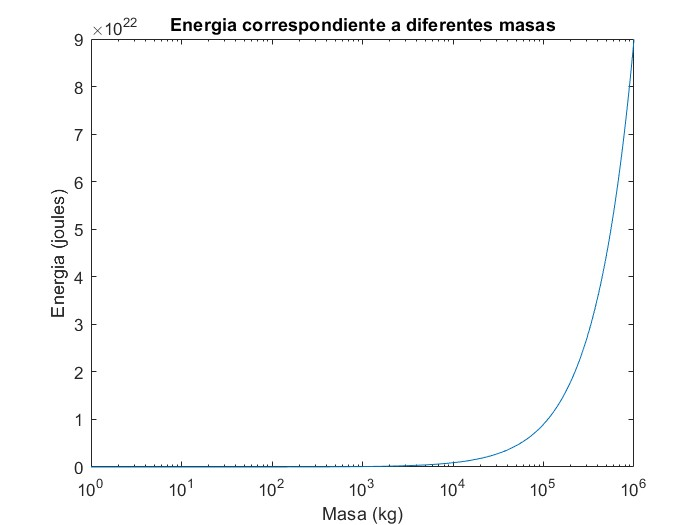
\includegraphics[width=\textwidth]{img8.jpg}
	\end{figure}
	
	\newpage
	\subsection{height}
	
	Un cohete se lanza verticalmente. En el tiempo $t = 0$, el motor del cohete se apaga. En ese momento, el cohete ha alcanzado una altura de 500 metros y se eleva con una velocidad de 125 metros por segundo. Entonces la gravedad toma el control. La altura del cohete como función del tiempo es:
	
	$$h(t) = -\frac{9.8}{2}t^2 + 125t + 500 \qquad \text{para } t > 0$$
	\newline
	Cree una función llamada `height` que acepte un tiempo `t` como entrada y regrese la altura `h` del cohete.
	
	\subsubsection{Función}
	
	\begin{lstlisting}
		
		function h = height(t)
		% HEIGTH Calcula la altura del cohete en funcion del tiempo
		%
		% Entrada:
		% t - Tiempo
		%
		% Salida:
		% h - Altura
		
		if t <= 0
		
		h = 500;
		
		else
		
		h = -4.9 * t^2 + 125 * t + 500;
		
		end
		
		end
		
	\end{lstlisting}
	
	\subsubsection{Ejecución}
	
	\begin{lstlisting}
	>> height(10)
	
	ans =
	
	1260
	\end{lstlisting}
	
	\begin{lstlisting}
	>> height(20)
	
	ans =
	
	1.0400e+03
	\end{lstlisting}
	
	\begin{lstlisting}
	>> height(16)
	
	ans =
	
	1.2456e+03
	\end{lstlisting}
	
	\newpage
	Cree un programa que grafique $h(t)$ contra $t$ para tiempos desde 0 hasta 30 segundos. Use un incremento de 0.5 segundo en su vector tiempo.
	
	\subsubsection{Script}
	
	\begin{lstlisting}
		
		% Programa que grafica la funcion height
		
		t = 0:0.5:30;
		
		h = zeros(size(t));
		
		for i = 1:length(t)
		
		h(i) = height(t(i));
		
		end
		
		plot(t, h);
		
		xlabel('Tiempo (s)');
		
		ylabel('Altura (m)');
		
		title('Altura del Cohete en Funcion del Tiempo');
		
	\end{lstlisting}
	
	\subsubsection{Ejecución}
	
	\begin{lstlisting}
	>> programa9
	\end{lstlisting}
	
	\subsubsection{Grafica}
	
	\begin{figure}[H]
		\centering
		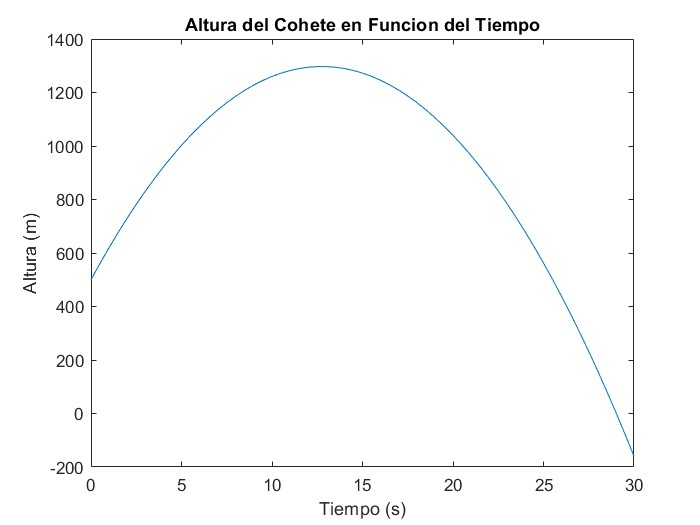
\includegraphics[height=11cm]{img9.jpg}
	\end{figure}
	
	\subsection{nmoles(m, MW)}
	
	En química de secundaria, se introduce la relación entre moles y masa:
	
	$n = \frac{m}{MW}$
	
	Donde
	$n$ es el número de moles de una sustancia,
	$m$ es la masa de la sustancia, y
	$MW$ es el peso molecular (masa molar) de la sustancia.
	
	Cree una función llamado \texttt{nmoles} que requiera dos entradas vectoriales (la masa y el peso molecular) y que regrese el correspondiente número de moles.
	
	\subsubsection{Función}
	
	\begin{lstlisting}
		
		function n = nmoles(m, MW)
		% NMOLES encuentra el numero de moles correspondiente a la masa y peso 
		% molecular dados
		%
		% Entradas:
		% m - vector de masa de la sustancia en gramos
		% MW - vector de peso molecular de la sustancia en g/mol
		%
		% Salida:
		% n - vector de numero de moles correspondientes a cada masa y peso 
		% molecular
		
		n = m ./ MW;
		
		end
	\end{lstlisting}
	
	\subsubsection{Ejecución}
	
	\begin{lstlisting}
	>> nmoles(12, 18.2)
	
	ans =
	
	0.6593
	\end{lstlisting}
	
	Escriba un programa que obtenga el numero de moles para los compuestos que se muestran en la siguiente tabla, para masas desde $1$ hasta $10 g$.
	\newline
	\begin{center}
		\begin{tabular}{|c|c|c|}
			\hline
			\textbf{Compuesto} & \textbf{Peso molecular (masa molar)} \\
			\hline
			Benceno & 78.115 g/mol \\
			\hline
			Alcohol etílico & 46.07 g/mol \\
			\hline
			Refrigerante R134a (tetrafluoroetano) & 102.3 g/mol \\
			\hline
		\end{tabular}
	\end{center}
	
	\newpage
	\subsubsection{Script}
	
	\begin{lstlisting}
		
		% Programa para calcular las masas de 1 a 10 gramos y imprimirlos en una
		% tabla.
		
		pesoMolecular = [78.115, 46.07, 102.3]; % g/mol
		compuestos = {'Benceno', 'Alcohol etilico', 'Refrigerante R134a'};
		nCompuestos = length(compuestos);
		
		masas = 1:10;
		nMasas = length(masas);
		
		resultados = zeros(nMasas, nCompuestos);
		
		for i = 1:nCompuestos
		for j = 1:nMasas
		resultados(j, i) = nmoles(masas(j)/1000, pesoMolecular(i));
		end
		end
		
		disp('Numero de moles para masas de 1 a 10 gramos:')
		fprintf('%-10s%-20s%-20s%-20s\n', 'Masa (g)', compuestos{:})
		for i = 1:nMasas
		fprintf('%-10.0f%-20.3e%-20.3e%-20.3e\n', masas(i), resultados(i,:))
		end
		
	\end{lstlisting}
	
	\subsubsection{Ejecución}
	
	\begin{lstlisting}
	>> Programa10
	Numero de moles para masas de 1 a 10 gramos:
	Masa (g)  Benceno             Alcohol etilico     Refrigerante R134a  
	1         1.280e-05           2.171e-05           9.775e-06           
	2         2.560e-05           4.341e-05           1.955e-05           
	3         3.840e-05           6.512e-05           2.933e-05           
	4         5.121e-05           8.682e-05           3.910e-05           
	5         6.401e-05           1.085e-04           4.888e-05           
	6         7.681e-05           1.302e-04           5.865e-05           
	7         8.961e-05           1.519e-04           6.843e-05           
	8         1.024e-04           1.736e-04           7.820e-05           
	9         1.152e-04           1.954e-04           8.798e-05           
	10        1.280e-04           2.171e-04           9.775e-05  
	\end{lstlisting}
	
	\newpage
	\section{Conclusión}
	
	En conclusión, esta práctica busca fortalecer las habilidades de programación en MATLAB y aplicarlas en distintas funciones matemáticas para resolver problemas en el mundo real. La implementación de funciones permite la reutilización de código y facilita la solución de problemas repetitivos en distintos contextos.
	
\end{document}